% Chapter Template

\chapter{Ensayos y Resultados} % Main chapter title

\label{Chapter4} % Change X to a consecutive number; for referencing this chapter elsewhere, use \ref{ChapterX}

%----------------------------------------------------------------------------------------
%	SECTION 1
%----------------------------------------------------------------------------------------

%\section{Pruebas funcionales del hardware}
%\label{sec:pruebasHW}

%La idea de esta sección es explicar cómo se hicieron los ensayos, qué resultados se obtuvieron y analizarlos.

\section{Validación de grafos}
	
	\subsubsection{Topología bypass}
	\subsubsection{Topología playa de maniobras}
	\subsubsection{Topología estación}
	
	
	\begin{figure}[h]
	\centering
	%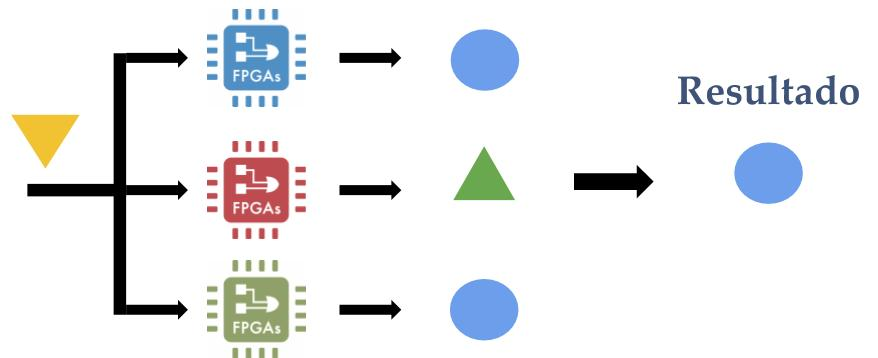
\includegraphics[scale=.3]{./Figures/Redundancia}
		\caption{HOLA}
		\label{fig:hola}
	\end{figure}
	\improvement{Incluir figura}
		
\section{Validación del nodo}

	\begin{figure}[h]
	\centering
	%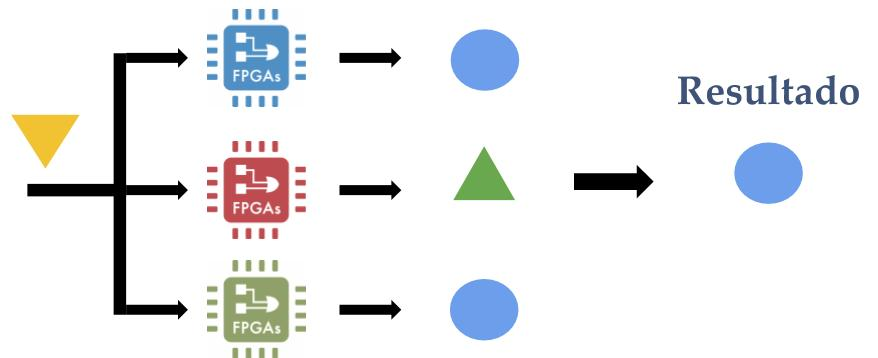
\includegraphics[scale=.3]{./Figures/Redundancia}
		\caption{HOLA}
		\label{fig:hola}
	\end{figure}
	\improvement{Incluir figura}
	
\section{Validación de la máquina de cambios}

	\begin{figure}[h]
	\centering
	%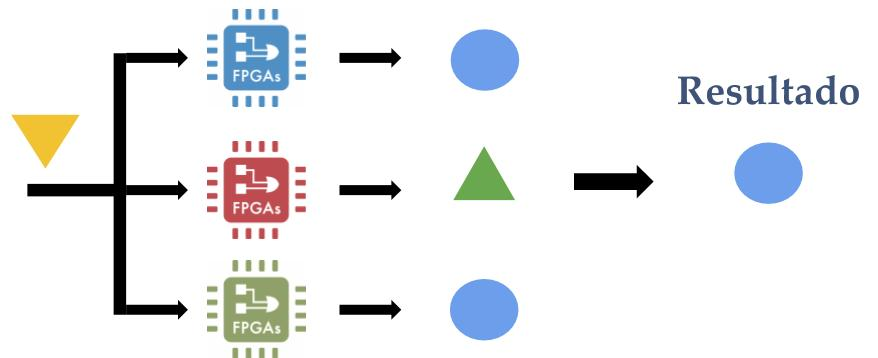
\includegraphics[scale=.3]{./Figures/Redundancia}
		\caption{HOLA}
		\label{fig:hola}
	\end{figure}
	\improvement{Incluir figura}
	
\section{Validación de la red}

	\begin{figure}[h]
	\centering
	%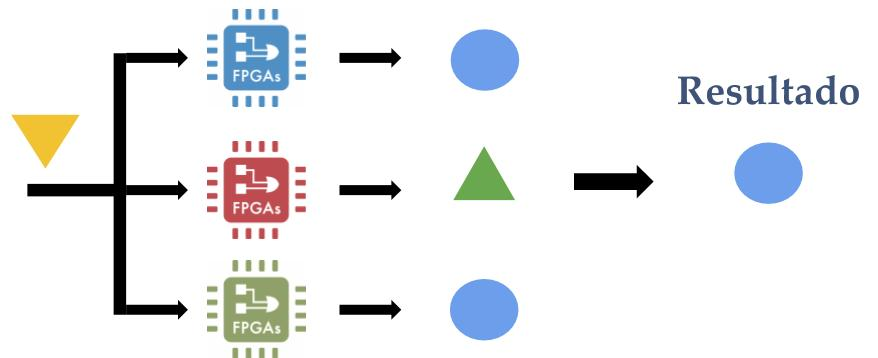
\includegraphics[scale=.3]{./Figures/Redundancia}
		\caption{HOLA}
		\label{fig:hola}
	\end{figure}
	\improvement{Incluir figura}
	
\section{Validación de la UART}

	\begin{figure}[h]
	\centering
	%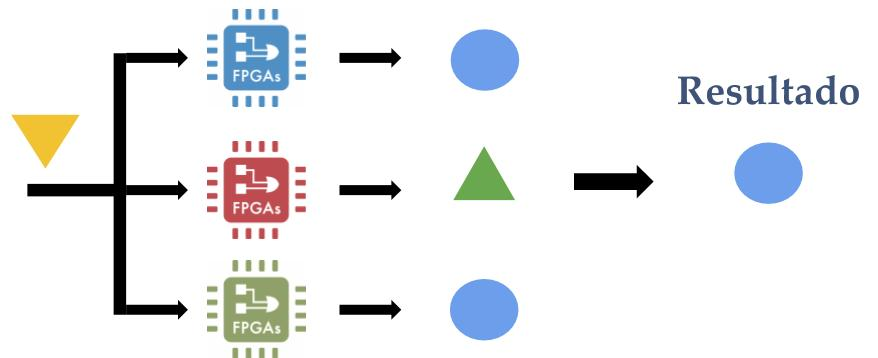
\includegraphics[scale=.3]{./Figures/Redundancia}
		\caption{HOLA}
		\label{fig:hola}
	\end{figure}
	\improvement{Incluir figura}
	
\section{Validación del sistema}

	\begin{figure}[h]
	\centering
	%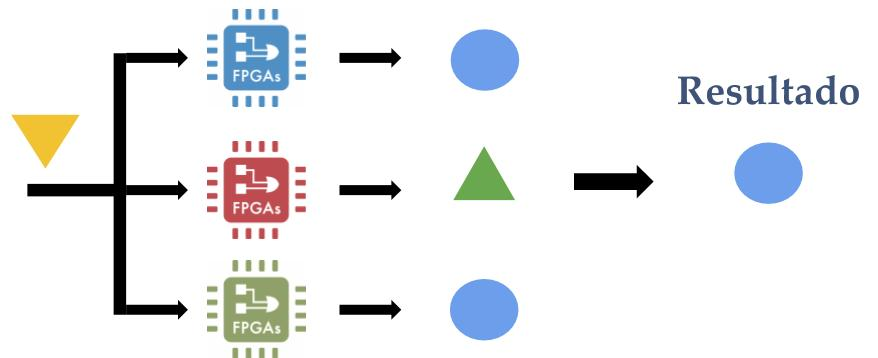
\includegraphics[scale=.3]{./Figures/Redundancia}
		\caption{HOLA}
		\label{fig:hola}
	\end{figure}
	\improvement{Incluir figura}